%<dscrpt>Plans médiateur, bissecteur et hauteur d'un triangle dans l'espace.</dscrpt>
On se place dans l'espace euclidien usuel muni d'un repère fixé d'origine $O$. Ce repère aide pour la visualisation des figures mais \emph{aucun calcul de coordonnées n'est nécessaire}. Tous les plans et droites considérés contiennent le point $O$. On adopte les notations suivantes :
\begin{itemize}
\item $\mathcal{D}(\overrightarrow{u})$ est la droite de vecteur directeur $\overrightarrow{u}$.
\item $\mathcal{P}(\overrightarrow{u},\overrightarrow{v})$ est le plan contenant  et $\overrightarrow{v}$.
\item $\mathcal{P}(\overrightarrow{u}^\bot)$ est le plan orthogonal à $\overrightarrow{u}$.
\end{itemize}
Les notations utilisées pour désigner les points et les vecteurs respecteront les conventions suivantes :
\begin{itemize}
\item $M$ et un point et $\overrightarrow{m}$ un vecteur tels que $\overrightarrow{OM}=\overrightarrow{m}$.
\item $A$ et un point et $\overrightarrow{a}$ un vecteur tels que $\overrightarrow{OA}=\overrightarrow{a}$.
\item $U$ et un point et $\overrightarrow{u}$ un vecteur tels que $\overrightarrow{OU}=\overrightarrow{u}$.
\item $\cdots$
\end{itemize}
On se donne trois vecteurs $\overrightarrow{u}$, $\overrightarrow{v}$, $\overrightarrow{w}$ non nuls et non coplanaires. Pris deux à deux, ces vecteurs ne sont ni colinéaires ni orthogonaux. L'objet du problème est d'étudier (à l'aide de produits vectoriels) des configurations classiques dans le plan associées à un \og triangle\fg~ de l'espace formé par les trois droites $\mathcal{D}(\overrightarrow{a})$, $\mathcal{D}(\overrightarrow{b})$, $\mathcal{D}(\overrightarrow{c})$ .

\begin{enumerate}
\item Préliminaires
\begin{enumerate}
\item On considère trois vecteurs $\overrightarrow{a},\overrightarrow{b},\overrightarrow{c}$ non nuls, non colinéaires et tels que
\[\overrightarrow{a}\wedge\overrightarrow{b}\neq \overrightarrow{0}, \quad \overrightarrow{a}+\overrightarrow{b}+\overrightarrow{c}=\overrightarrow{0}\]
Montrer que
\[\mathcal{P}(\overrightarrow{a}^\bot) \cap \mathcal{P}(\overrightarrow{b}^\bot) \cap \mathcal{P}(\overrightarrow{c}^\bot) = \mathcal{D}(\overrightarrow{a}\wedge\overrightarrow{b})\]
\item Former l'équation normale d'un plan $\mathcal{P}(\overrightarrow{a},\overrightarrow{b})$ et préciser la distance d'un point $M$ à ce plan. (question de cours, la démonstration n'est pas demandée)
\end{enumerate}

\begin{figure}[ht]
   \centering
   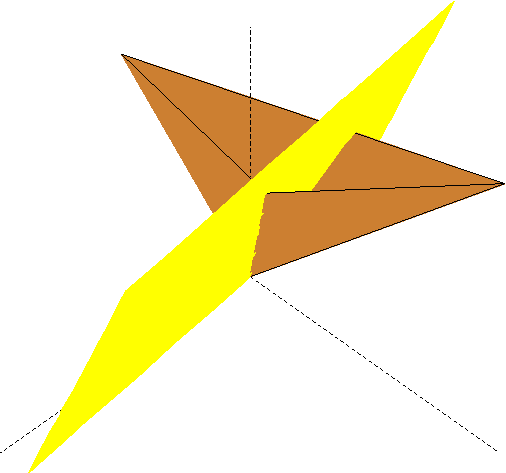
\includegraphics[width=6cm]{Etriproj_1.pdf}
   \caption{Plan \og hauteur\fg.}
   \label{fig:Etriproj_1}
\end{figure}

\item Plans \og hauteurs\fg~ du triangle dans l'espace.\newline
On définit le plan \og hauteur\fg~ issu de $\overrightarrow{u}$ comme étant orthogonal à $\mathcal{P}(\overrightarrow{v},\overrightarrow{w})$ et contenant $\mathcal{D}(\overrightarrow{u})$.
\begin{enumerate}
\item Former un vecteur orthogonal au plan \og hauteur\fg~ issu de $\overrightarrow{u}$.

\item Montrer l'identité (dite de Jacobi):
\[
(\overrightarrow{u} \wedge \overrightarrow{v})\wedge \overrightarrow{w} +
(\overrightarrow{v} \wedge \overrightarrow{w})\wedge \overrightarrow{u} +
(\overrightarrow{w} \wedge \overrightarrow{u})\wedge \overrightarrow{v}
= \overrightarrow{0}\]
En déduire que l'intersection des trois plans \og hauteurs\fg~ est une droite. Cette droite est notée $\mathcal{D}_h$.
\end{enumerate}

\begin{figure}[ht]
   \centering
   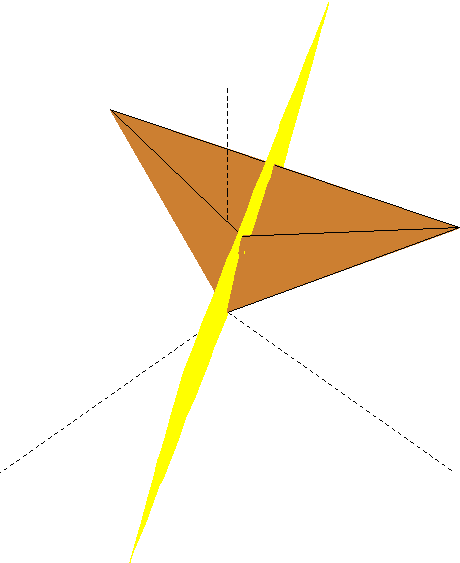
\includegraphics[width=6cm]{Etriproj_2.pdf}
   \caption{Plan \og bissecteur\fg.}
   \label{fig:Etriproj_2}
\end{figure}

\item Plans \og bissecteurs\fg~ du triangle dans l'espace.
\begin{enumerate}
\item Montrer que l'ensemble des points équidistants de deux plans $\mathcal{P}(\overrightarrow{u},\overrightarrow{v})$ et $\mathcal{P}(\overrightarrow{w},\overrightarrow{u})$ est la réunion de deux plans.
\item Former un vecteur orthogonal pour chacun de ces deux plans.\newline
Parmi ces deux vecteurs, un seul (noté $\overrightarrow{a}$) est tel que $\overrightarrow{a} . \overrightarrow{v}$ et $\overrightarrow{a} . \overrightarrow{w}$ soient de signes opposés. Préciser ce vecteur $\overrightarrow{a}$.\newline
On dit que $\mathcal{P}(\overrightarrow{a}^\bot)$ est le \emph{plan bissecteur intérieur issu de $\overrightarrow{u}$}.\newline
Les deux autres plans bissecteurs intérieurs (issus de $\overrightarrow{v}$ et $\overrightarrow{w}$) s'obtiennent par permutation des lettres.
\item Préciser $\overrightarrow{b}$ et $\overrightarrow{c}$. Montrer que l'intersection des trois plans est une droite. Cette droite est notée $\mathcal{D}_b$.
\end{enumerate}

\begin{figure}[ht]
   \centering
   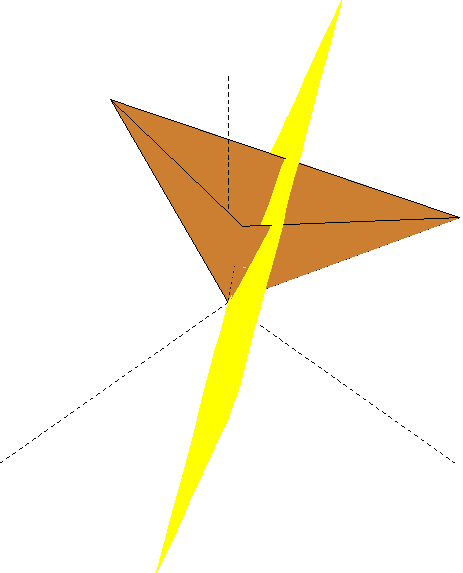
\includegraphics[width=6cm]{Etriproj_3.pdf}
   \caption{Plan \og médiateur\fg.}
   \label{fig:Etriproj_3}
\end{figure}

\item Plans \og médiateurs\fg~ du triangle dans l'espace.
\begin{enumerate}
\item Montrer qu'un point $M$ est équidistant des droites $\mathcal{D}(\overrightarrow{v})$ et $\mathcal{D}(\overrightarrow{w})$ si et seulement si il est équidistant des plans $\mathcal{P}(\overrightarrow{v}^\bot)$ et $\mathcal{P}(\overrightarrow{w}^\bot)$.
\item Montrer que l'ensemble des points équidistants des deux droites $\mathcal{D}(\overrightarrow{v})$ et $\mathcal{D}(\overrightarrow{w})$ est la réunion de deux plans.
\item Former un vecteur orthogonal pour chacun de ces deux plans.\newline
Parmi ces deux vecteurs, un seul (noté $\overrightarrow{a}$) est tel que $\overrightarrow{a} . \overrightarrow{v}$ et $\overrightarrow{a} . \overrightarrow{w}$ soient de signes opposés. Préciser ce vecteur $\overrightarrow{a}$.\newline
On dit que $\mathcal{P}(\overrightarrow{a}^\bot)$ est le \emph{plan médiateur intérieur issu de $\overrightarrow{u}$}.\newline
Les deux autres plans médiateurs intérieurs (issus de $\overrightarrow{v}$ et $\overrightarrow{w}$) s'obtiennent par permutation des lettres.
\item Préciser $\overrightarrow{b}$ et $\overrightarrow{c}$. Montrer que l'intersection des trois plans est une droite. Cette droite est notée $\mathcal{D}_m$.

\end{enumerate} 

\item Préciser pour chacun des trois vecteurs suivants
\begin{eqnarray*}
\frac{\overrightarrow{u}\wedge \overrightarrow{v}}{\Vert \overrightarrow{u}\Vert \Vert \overrightarrow{v} \Vert} +
\frac{\overrightarrow{v}\wedge \overrightarrow{w}}{\Vert \overrightarrow{v}\Vert \Vert \overrightarrow{w} \Vert} +
\frac{\overrightarrow{w}\wedge \overrightarrow{u}}{\Vert \overrightarrow{w}\Vert \Vert \overrightarrow{u} \Vert} \\
\Vert \overrightarrow{v}\wedge \overrightarrow{w} \Vert \overrightarrow{u} +
\Vert \overrightarrow{w}\wedge \overrightarrow{u} \Vert \overrightarrow{v} +
\Vert \overrightarrow{u}\wedge \overrightarrow{v} \Vert \overrightarrow{w} \\
\dfrac{\overrightarrow{u}\wedge \overrightarrow{v}}{\overrightarrow{u}. \overrightarrow{v}} +
\dfrac{\overrightarrow{v}\wedge \overrightarrow{w}}{\overrightarrow{v}. \overrightarrow{w}} +
\dfrac{\overrightarrow{w}\wedge \overrightarrow{u}}{\overrightarrow{w}. \overrightarrow{u}}
\end{eqnarray*}
la droite parmi $\mathcal{D}_b$, $\mathcal{D}_m$, $\mathcal{D}_h$ dont il est un vecteur directeur.
\end{enumerate}
\clearpage